
\chapter{La visibilità}

Altra caratteristica essenziale per l'informazione all'interno di un sito è l'essere trovata. Per far ciò conta la \textbf{visibilità esterna} e questa è determinata dal posizionamento del sito sui motori di ricerca. 
	Vedremo che è essenziale posizionarsi nella top 10 per le \emph{keyword} che ci riguardano e capiremo come promuovere un sito analizzando il funzionamento dei \emph{search engine} (SE) e l'uso che gli utenti ne fanno.

	\section{Posizionamento SERP}	
		La top 10 risultati assorbe il 95\% dei click dell'utenza dopo una ricerca.
		\begin{enumerate}
			\item 51\% click (il primo risultato prende più di tutte le altre!),
			\item 16\% click;
			\item 6\% click;
			\item 6\% click;
			\item 5\% click;
			\item 4\% click;
			\item 2\% click;
			\item 1\% click;
			\item 1\% click;
			\item 2\% click (effetto \emph{black jersay} o \emph{Malabrocca}).		
		\end{enumerate}
		
		Nota: le strategie che verranno illustrate in seguito non funzionano sempre, basta infatti un minimo cambiamento per cambiare il comportamento degli utenti sui risultati. Infatti recenti introduzioni di Google sono state analizzate molto, prima di farle diventare effettive. La striscia di immagini per esempio svolgono un effetto sospensivo per trattenere l'utente e non hanno impatto sulla percezione del testo.
	
	\section{SPAMDEX (SEO)}
		È l'insieme di attività svolte con lo scopo di far sì che un sito sia indicizzato da Google e occupi le posizioni più alte della SERP. Nelle seguenti sezioni prima spiegheremo il funzionamento dei motori di ricerca e poi illustreremo le tecniche per migliorare il posizionamento o addirittura ingannare il SE.
		Il \textbf{punteggio di una pagina} è calcolato sul riferimento a due componenti delle pagine:
		\begin{itemize}
			\item componente \textbf{testuale};
			\item componente \textbf{ipertestuale}.
		\end{itemize}
		
		\subsection{Parte testuale}
			Per la parte testuale si misura la qualità in base a quanto una parola è importante per una pagina attraverso il TFIDF. Per misurare l'importanza di una parola si utilizzano due tecniche:
			
			\subsubsection{Term frequency (TF)}
				Misurare la frequenza di una parola. Ad esempio su 100 parole in una pagina 5 sono di nostro interesse per cui il TF è uguale al 5\%.
				È ovvio che solo questa tecnica non basta per avere risultati soddisfacenti, parole molto frequenti come articoli, congiunzioni, eccetera avrebbero un'importanza troppo alta anche se prive di significato.
				
			\subsubsection{Inverse document frequency}
				È la misura dell'inverso della frequenza della parola nell'insieme dei documenti (il sito web) scalata logaritmicamente. 
				
				Esempio: su 1000 pagine "il" appare in 980 pagine, ha TF=98\% mentre:
				\[
					IDF=\log \left(\frac{1}{0,98} \right)=0,008;
				\]
				
				Altro esempio: su 1000 pagine la parola "pippo" ha il 10\% di frequenza, allora:
				\[
				IDF=\log \left(\frac{1}{0,1} \right)=1;
				\]
				
				Ora più rara è la parola più è alto il bonus.
				
			\subsubsection{Query SE}
				Ogni \emph{query} sarà composta dalle parole con cui il SE andrà a calcolare TF e IDF nei siti web. Quelli con il valore più alto si posizioneranno più in alto.
				Se sottoponiamo una \emph{query} con una parola $p$  il SE prende le pagine dove appare $p$ e ne calcola il TF e l'IDF. Per più parole in una \emph{query} si usa la somma del TF e IDF.
				In questo modo alzare il punteggio di una parola può rischiare di diluire il valore e viceversa. È importante quindi selezionare un gruppo di parole e alzare il loro TFIDF a scapito di altre, queste \emph{keyword} saranno le parole che competeranno nella SERP.
			
		\subsection{Term spam}
			Vediamo quindi alcune tecniche per aumentare il punteggio per le \emph{keyword} definite.
			\begin{description}
				\item[Body spam:] inserire le \emph{keyword} semplicemente nel body html.
				\item[Title spam:] inserire le \emph{keyword} sul titolo delle pagine web, è una parte che l'utenza media non vedrà mai.
				\item[Meta tag spam:] inserire le \emph{keyword} in appositi tag html (i \emph{meta}) che descrivono a \emph{keyword} la pagina. Per l'inteso sfruttamento i SE oramai ignorano questo genere di spam.
				\item[Anchor text spam:] inserire le \emph{keyword} nel testo di un link tra i tag \verb|<a>...</a>|. Questo oltre al punteggio della pagina aumenta il punteggio alla pagina destinazione e il bonus viene dato con meno limiti per il TFIDF.
				\item[URL spam:] inserire le \emph{keyword} nell'URL dell'indirizzo della pagina. Otteniamo bonus simili a quelli dell'\emph{anchor text spam}.
			\end{description}
			
		
			\subsubsection{Starter kit}
				Abbiamo visto dove inserire le \emph{keyword}. Ora vediamo le tecniche utilizzate di come inserirle:
				\begin{description}
					\item[Repetition:] ripetere la \emph{keyword} stando attenti al suo TFIDF. Tecnica facile da trovare dal SE che può pure penalizzare.
					\item[Dumping:] inserire termini rari nel testo anche se non c'entrano nulla. Otteremo un punteggio alto sul sito anche se questo non è pertinente.
					\item[Weaving:] utilizzare pezzi di altre pagine web in cui sono inserite le nostre \emph{keyword} in modo random.
					\item[Stitching:] \emph{past \& copy} da siti differrenti e si assembla il tutto ottenendo un contenuto rilevante. Per esempio da una risposta di un utente su un forum sviluppiamo un articolo nuovo. Più argomenti diversi danno inoltre un bonus globale e i SE fanno fatica a capire se è contenuto copiato.
					\item[Broadening:] oltre alle \emph{keyword} fare uso di sinonimi e frasi correlate. Questo coprirà più le \emph{query} degli utenti.
				\end{description}		
		
			\subsubsection{Quali keyword?}
				Una domanda di cui la risposta probabilmente decreterà il successo di un sito. Le \emph{keyword} devono essere pensate in base a quello che cerca l'utente. Occorre un'attenta analisi prima di lanciarsi nel mondo SEO. Di seguito alcuni strumenti utili a tale scopo:
				\begin{itemize}
					\item \href{https://adwords.google.com/KeywordPlanner}{Google keyword tool} (a pagamento);
					\item \href{http://keywordtool.io/}{keywordtool.io} (alternativa gratis);
					\item \href{https://www.google.it/trends/}{Google Trends} (ottimo per capire la tendenza nel tempo);
				\end{itemize}
			
		\subsection{Problema e soluzioni del term spamming}
			Non basta potenziare la pagina, se infatti questa non è utile e soffre di problemi di usabilità l'utente semplicemente abbandonerà. Se vogliamo potenziare una pagina con le tecniche di \emph{term spamming} dobbiamo nascondere in qualche modo all'utente ciò che serve ai SE.
		
			\subsubsection{Content hiding}
				Il contenuto potenziante è nascosto all'utente e solo i motori di ricerca lo vedono.
			
			\subsubsection{Redirection}
				Anche detta tecnica 302, consiste nel potenziare una pagina che sarà costruita con soli fini di posizionamento che indirizza alla vera pagina. In questo modo gli utenti vedranno la pagina studiata per loro mentre i SE si fermeranno a leggere la prima. Questa tecnica funziona solo con trucchetti che richiedono \emph{javascript}, il \emph{meta} che reindirizza infatti è riconosciuto dai SE. Con l'uso di \emph{javascript} il \emph{meta} verrà aggiunto dinamicamente e i SE, per costi di risorse, non si accorgeranno poiché non eseguono il codice. Tuttavia ad oggi i SE leggono il codice \emph{javascript} e cercano se esiste questa tecnica, per ingannarli è sufficiente offuscare un po' il codice.
			
			\subsubsection{Cloaking}
				Controlla l'accesso alla pagina per capire se chi visita è un bot o un umano. Se questo è un bot li presento una pagina apposita diversa da quella mostrata all'utente. È una tecnica difficile da scoprire tanto che Google la penalizza moltissimo se segnalata ma questo avviene solo tramite intervento umano.
			
	
		\subsection{Parte ipertestuale: pagerank}
			Il punteggio delle pagine web è affidato anche ai link di ipertesto: il \emph{pagerank}. Ad ogni pagina $\pi_v$ era affidato un punteggio pari a:
				\[
					\pi_v=\sum_{(\omega, v) \in E}\frac{\pi_{\omega}}{d_w}
				\]
			Dove:
			\begin{itemize}
				\item $\omega$, $v$ è un link da $\omega$ a $v$;
				\item $d_\omega$ è il numero di link uscenti.
			\end{itemize}
			Ossia, se una pagina $\omega$ ha un link verso un'altra pagina viene data una frazione ($1/d_\omega$) di \emph{pagerank} a quest'ultima.
			Come vincolo abbiamo:
			\[
				\sum\pi_v=1
			\]
			
			Questo calcolo di \emph{pagerank} molto naive era molto facile da manipolare con gli stratagemmi visti in precedenza, si è deciso quindi di farne una riformulazione.
		
			\subsubsection{Le catene di Markov e il random walk}
				La riformulazione avviene sfruttando l'algebra lineare e speciali matrici dette catene di Markov che godono di alcune proprietà unite alla teoria della probabilità. Il \emph{pagerank} di una pagina web diventa quindi la probabilità di entrare in quella pagina da altre pagine.
				Per rendere più chiaro il concetto si può pensare ad una scimmia  (un \emph{random surfer}) che naviga il web in modo del tutto casuale, la probabilità che la scimmia entri in una pagina ne determina il suo punteggio.
				
				Esempio:
					dato il seguente grafo i nodi che rappresentano pagine e gli archi i link:
					$A \longleftrightarrow B \longleftrightarrow C$,
					
					B ottiene il 50\% del flusso mentre A e C il 25\%.
					
				Il \emph{random surfer} è un altro fattore su cui tener conto ma attenzione esso non rispecchia esattamente gli intenti degli utenti che non navigano totalmente a caso.
			
			\subsubsection{Problemi: spider traps e island}
				Per attuare il sistema spiegato in precedenza c'è la necessità di far girovagare questi \emph{random surfer} (i famosi \emph{spider}) che raccolgono dati da cui calcolare il \emph{pagerank}. La navigazione casuale da pagina a pagina può rivelarsi fatale in alcuni casi.
				\begin{description}
					\item[Spider traps:] nel caso in cui uno spider rimanga intrappolato all'interno di un sito in cui pagine continuano a indirizzare ad altre pagine in un ciclo infinito (si pensi ad un calendario online).
					\item[Island:] esistono poi casi in cui alcuni pezzi di rete sono isolati dagli altri, dei veri e propri micro-web indipendenti in cui per gli \emph{spider} non c'è alcun modo di passare, ciò significa: nessun valore di \emph{pagerank} o infiniti valori diversi di \emph{pagerank}.
				\end{description}
				
		\subsection{Pagerank 2.0}
			A seguito dei problemi prima elencati si è cercato un'altra soluzione: il teletrasporto. La formula quindi cambia in (con $N$ numero totale di pagine):
			\[
				\pi_v=(1-\epsilon)\cdot \left( \sum_{\omega, v \in E} \frac{\pi_{\omega}}{d_w} \right) + \frac{\epsilon}{N}
			\]
			Nella pratica si è aumentata la casualità. Ora la scimmia ha anche un dado,  con una certa probabilità effettua il teletrasporto in un'altra pagina casuale altrimenti fa come spiegato in precedenza (da notare un comportamento apparentemente più strano se paragonato con quello degli utenti, in realtà non poi così tanto poiché molte volte un utente effettua il teletrasporto attraverso URL diretto).
			
			In questo modo grazie al \textbf{fattore di teleporting} $\epsilon$ risolviamo \emph{spider traps} e \emph{island}; più questo fattore è verso il 100\% e più il punteggio in probabilità alle pagine diventa uguale per tutte, viceversa più è verso lo 0 e più il \emph{pagerank} si avvicina a quello calcolato in precedenza.
			
			Un altro modo per il calcolo del \emph{pagerank} è il \emph{total rank}:
			\[
				T=\int_0^1r(\alpha) d\alpha
			\]
			
		
			\subsubsection{Problema: dead ends}
				Nonostante l'introduzione del teletrasporto rimane il problema (prima non illustrato) delle \emph{dead ends}. Con questa formula l'egoismo paga, un sito è meglio che mantenga i link al suo interno.
				
				La soluzione a cui sono arrivati i moderni motori di ricerca è calcolare l'importanza su altro per ogni sito e pagina web e non sul vero web. (vedere paragrafo ~\ref{sec:email})
		
		\subsection{Migliorare il pagerank}
			Esistono due fattori fondamentali che influenzano il \emph{pagerank} con l'uso del teletrasporto:
			\begin{itemize}
				\item Inlink;
				\item Outlink.
			\end{itemize}
		
			\subsubsection{Inlink}
				Link entranti alla pagina. Per incrementare il \emph{pagerank} di una pagina dobbiamo fare in modo che questa sia puntata dal maggior numero di pagine esterne. Alcune tecniche per fare ciò sono:
				\begin{description}
					\item[Infiltration:] infiltrarsi in altri siti e mettere link alla pagina da potenziare (commenti spam etc.).
					\item[Honey pot:] creare contenuto appetibile e utile che riceve link (è il modo giusto di aumentare il \emph{pagerank}). Molto spesso questo contenuto è vittima del \emph{copy \& past}.
					\item[Link exchange:] allearsi con altri per scambiarsi link.
					\item[Resurrection:] acquistare domini defunti con \emph{pagerank} abbastanza alto. Il \emph{pagerank} infatti non decade mai e resta legato al dominio, inoltre l'età del dominio conta come bonus. Esistono interi business per la vendita di domini defunti ma appetibili per il proprio \emph{pagerank}.
				\end{description}
				
				\paragraph{Marketing 2.0}
					Un esempio nella storia del web di quanto siano importanti gli \emph{inlink} arriva dalla pagina \href{http://www.milliondollarhomepage.com/}{million dollar page}. Una schermata di pixel venduta a 1 dollaro l'uno, il punto forte per cui tutti si affrettarono di acquistare almeno 1 pixel fu la presenza di tutti i link che puntavano alla pagina resa famosa dall'originale idea dell'autore. La pagina diventò una vera e propria cascata di flusso per il \emph{pagerank} ed ogni link al suo interno ne acquistava un po' ad un prezzo ridicolo.
			
			\subsubsection{Outlink}
				Passiamo ora ai link uscenti. Posizionando un link esterno in una pagina un po' di flusso di \emph{pagerank} esce dalla pagina. In questo modo è garantita la \textbf{solidità}, l'aggiunta di \emph{outlink} non alza il punteggio e lo \emph{smapdex} non può essere locale.
				Questo controintuitivamente non risulta essere vero! Con la presenza di \emph{outlink} posso aumentare il \emph{pagerank} della mia pagina con dinamiche imprevedibili. Ciò deriva dalla presenza del \emph{fattore di teleporting}.
			
			\subsubsection{Spam farm}
				Esistono numerose tecniche per usare gli \emph{outlink} e gli \emph{inlink} per aumentare il \emph{pagerank}. Le \emph{spam farm} sono una di queste tecniche: strutture apposite studiate di link e pagine per l'incremento del punteggio nei vari SE. 
				Una \emph{spam farm} ottimale singola consiste in una pagina o più pagine, definite pagine \textbf{target}, puntate da link bidirezionali da altre pagine, definite pagine \textbf{potenzianti}. Un struttura ottimale inoltre presenta la proprietà di \emph{reachability}, ovvero se gli spider dei SE raggiungono la pagina \emph{target} attraverso una pagina \emph{potenziante} allora tutta la \emph{spam farm} diventa raggiungibile (vedere figura ~\ref{fig:LaVisibilita-SpamFarm1}).
				
				\begin{figure} [h]
					\centering
					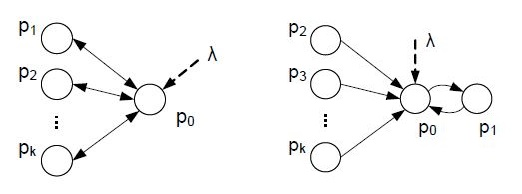
\includegraphics[scale=0.9]{images/LaVisibilita-SpamFarm1}
					\caption{La visibilità - Esempi spam farm singole ottimali}
					\label{fig:LaVisibilita-SpamFarm1}
				\end{figure}
				
				\paragraph{Alleanze}
					Il modo migliore per sfruttare le \emph{spam farm} è sfruttare alleanze con altri siti internet. Le alleanze tra siti (due e più) possono essere di tipo:
					\subparagraph{Alleanza profonda}
						Le pagine target distribuiscono il flusso sulle pagine potenzianti dell'altro sito (figura ~\ref{fig:LaVisibilita-SpamFarm2}) creando una media dei \emph{pagerank} stabile.
						
					\begin{figure} [h]
						\centering
						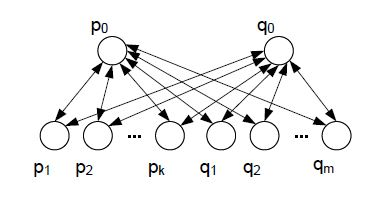
\includegraphics[scale=0.9]{images/LaVisibilita-SpamFarm2}
						\caption{La visibilità - Spam farm alleanza profonda}
						\label{fig:LaVisibilita-SpamFarm2}
					\end{figure}
						
					\subparagraph{Alleanza superficiale}
						Le pagine target dei due siti sono connesse con link (figura ~\ref{fig:LaVisibilita-SpamFarm3}, il \emph{pagerank} ottenuto risulta essere più del massimo delle due pagine target prima della connessione.
					
				\begin{figure} [h]
					\centering
					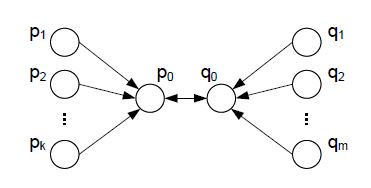
\includegraphics[scale=1]{images/LaVisibilita-SpamFarm3}
					\caption{La visibilità - Spam farm alleanza superficiale}
					\label{fig:LaVisibilita-SpamFarm3}
				\end{figure}
				
					\subparagraph{Alleanze Ring}
						Alleanza che comprende più di due siti. Le pagine target indicizzano in un percorso circolare la pagina target successiva creando una sorta di anello (figura ~\ref{fig:LaVisibilita-SpamFarm4}).
						
				\begin{figure} [h]
					\centering
					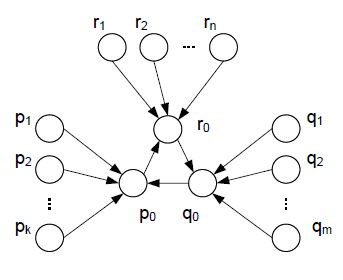
\includegraphics[scale=1]{images/LaVisibilita-SpamFarm4}
					\caption{La visibilità - Spam farm alleanza ring}
					\label{fig:LaVisibilita-SpamFarm4}
				\end{figure}
				
					\subparagraph{Alleanza complete core}
						Potenziamento della \emph{spam farm} di tipo \emph{ring}, la struttura bidirezionale è più vantaggiosa. Ora ogni pagina target ha link entrante e uscenti verso le due pagine target più vicine (figura ~\ref{fig:LaVisibilita-SpamFarm5}). Per fare un core basta un grafo fortemente connesso.
				
				\begin{figure} [h]
					\centering
					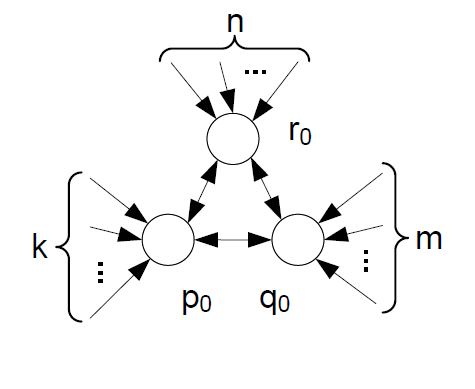
\includegraphics[scale=0.6]{images/LaVisibilita-SpamFarm5}
					\caption{La visibilità - Spam farm alleanza complete core}
					\label{fig:LaVisibilita-SpamFarm5}
				\end{figure}
				
			\subsubsection{Contromisure SE}
				Ovviamente le \emph{spam farm} sono azioni penalizzate dai SE poiché ingannano la misura del \emph{pagerank}. I motori di ricerca controbattono quindi cercando di identificare queste unioni rivelando l'esistenza di grafi fortemente connessi. Questi grafi dipendono dal modo con cui l'alleanza si è creata e dal numero di partecipanti ad asse. Visto il numero enorme di combinazioni fu creata un'enciclopedia delle sequenze. Purtroppo in ogni sequenza il numero di collegamenti da controllare cresce enormemente in base al numero di partecipanti (N), per:
				\begin{itemize}
					\item N=3 $\rightarrow$ 18 collegamenti;
					\item N=4 $\rightarrow$ 1606 collegamenti;
					\item N=5 $\rightarrow$ 565080 collegamenti;
					\item \dots
				\end{itemize}
				Non esiste nessuna formula che calcoli il risultato di collegamenti dato un numero N di partecipanti. Inoltre il costo computazionale risulta dispendiosissimo. Si sono quindi cercate soluzioni "laterali" più sofisticate.
				
				Un modo consiste in calcolare il vecchio \emph{pagerank} e confrontarlo con quello nuovo. Se il rapporto tra le due misure risulta troppo alto significa che la pagina analizzata è potenziata. È stato stimato che il successo di questa tecnica si trova tra il 95\% e 100\%.				
				
				Un altro modo consiste nel basarsi sulla \textbf{forma del web}: la struttura di alto livello a papillon (figura ~\ref{fig:LaVisibilita-FormaWeb}). L'idea è di analizzare la forma di un sito web, se questa non rispecchia ed ha valori al di fuori della media nella norma globale dei siti web allora il sito è sospetto e avviene un controllo più approfondito.
				Nella figura ~\ref{fig:LaVisibilita-ContromisureSE1} vediamo la zona creata dai link entranti nei siti nel web globale che rappresenta la norma. I punti situati all'esterno (evidenziati dall'ellisse) sono siti di cui si sospetta il potenziamento. Nella figura ~\ref{fig:LaVisibilita-ContromisureSE2} invece vediamo i link uscenti. 
				
				\begin{figure}
					\centering
					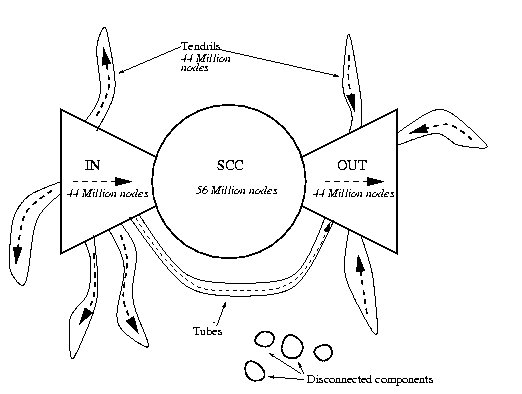
\includegraphics[scale=0.6]{images/LaVisibilita-FormaWeb}
					\caption{La visibilità - Forma ad alto livello del web}
					\label{fig:LaVisibilita-FormaWeb}
				\end{figure}								
				
				\begin{figure} [h]
					\subfloat[][\emph{Distribuzione link entranti}.]
						{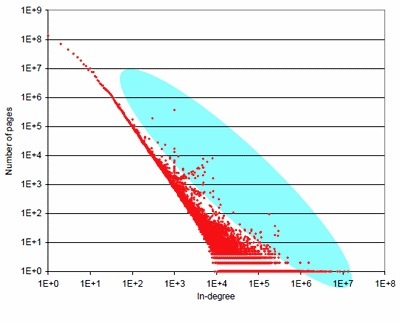
\includegraphics[width=.48\textwidth]{images/LaVisibilita-ContromisureSE1}
						\label{fig:LaVisibilita-ContromisureSE1}} \quad
					\subfloat[][\emph{Distribuzione link uscenti}.]
						{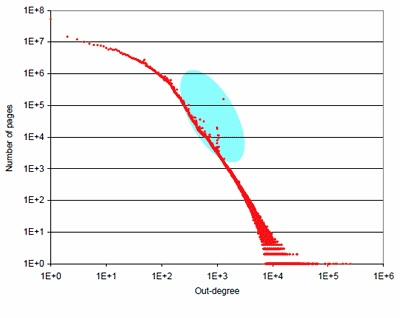
\includegraphics[width=.48\textwidth]{images/LaVisibilita-ContromisureSE2}
						\label{fig:LaVisibilita-ContromisureSE2}}
					\caption{La visibilità - Rappresentazioni grafiche dei link nel web}
					
				\end{figure}
			
		\subsection{Pagerank 3.0}
			Negli ultimi anni si è voluto migliorare la formula del \emph{pagerank} in particolare il fattore di teleporting.
			
			La vecchia formula (qui riporta in una versione leggermente diversa):
			\[
				(1-\epsilon )\cdot 1^T N + \epsilon L
			\]
			possiamo scriverla usando la matrice $P$ e diventa:
			\[
				(1- \epsilon )\cdot 1^T N + PL
			\]
			$P$ è una matrice che permette il \emph{pagerank} personalizzato che sostituisce il teletrasporto. Ogni nodo è pesato con preferenze così rendiamo il teletrasporto meno stupido. In questo modo però sorgono problemi riguardanti la libertà e la censura. Se infatti l'utente delle preferenze è il SE di turno, potrebbe volutamente alzare il \emph{pagerank} ad alcuni siti e abbassarlo ad altri. 
			
			È noto che Google personalizza la bontà di un sito, alcune sono addirittura fatte a mano! \emph{Searchking}, competitor di Google, è stato penalizzato in questo modo e il ricorso legale ha rivelato come il \emph{pagerank} sia soltanto un'opinione.
			Con questo nuovo livello di \emph{pagerank} quindi possiamo dichiarare defunta la democrazia contenuta in esso.
		
			\subsubsection{Pagerank personalizzato}
			
				Il \emph{pagerank} personalizzato però non è disponibile soltanto ai SE ma anche all'utente. Ogni profilo personale di ogni utente calcola un \emph{pagerank} personalizzato in base a tutti i dati raccolti su di lui (vedi tutte le piattaforme Google disponibili che ogni giorno utilizziamo tutti).  In questo modo i risultati di ricerca varieranno in base ai suoi interessi.
				Ma come calcolare questo \emph{pagerank} personalizzato per ogni utente nel web!? Se restringiamo a soli due valori: "sì" e "no" abbiamo con $N$ pagine: $2^N$ personalizzazioni. Troppe\dots
				Il \emph{pagerank} per fortuna ha la proprietà di essere \textbf{linearmente componibile} rispetto le probabilità; cioè se ho 100 pagine calcolate e risultanti "sì" e da un'altra parte ho altre 100 pagine calcolate e risultanti "sì" per calcolare il  \emph{pagerank} delle 200 pagine mi basta unire i risultati. Grazie a questa proprietà possiamo calcolare per $N$ pagine $N$ \emph{pagerank} personalizzati. Sono ancora troppi calcoli\dots $N$ è la taglia del web, miliardi di miliardi di pagine web!
				
				La soluzione quindi è il \emph{topic pagerank}, selezionare un certo numero di \emph{keyword} e \emph{topic}. Creare dei profili che approssimano gli utenti e su questo numero limitato calcolare il \emph{pagerank} personalizzato diviso a categorie a sua volta divise in \emph{topic} più precisi secondo le necessità. Combinando i \emph{pagerank} precalcolati traccio il profilo degli utenti. Da questi profili "grezzi" si calcolano i profili astratti che li conterranno e andranno a modificare il \emph{pagerank} in base alle ricerche dell'utente. Si fa notare che ogni \emph{pagerank} personalizzato è compatibile con le contromisure ma comporta disturbi e limitazioni alle ottimizzazioni SEO.
			
			\subsubsection{Bontà di una pagina: doppio ranking}
				Fino a poco tempo fa il \emph{pagerank} costituiva un punteggio positivo che coesisteva con le contromisure dei SE per penalizzarlo. 
				Le alterazioni e gli attacchi nel web però resero le contromisure non più sufficienti per questo si è deciso di affiancare al normale \emph{pagerank} positivo un \emph{pagerank} opposto: un punteggio negativo.
			
			\subsubsection{Janus Graph}
				Per ricorrere a questa nuova misura bisognava mantenere il modello sottostante sempre uniforme e semplice, si è quindi ricorso al \textbf{grafo di Giano}.
				Il \emph{Janus Graph} è un grafo in cui ogni nodo ha due valori associati:
				\begin{itemize}
					\item $W^+$ per la parte positiva;
					\item $W^-$ per la parte negativa.	
				\end{itemize}	
				$W^+$ e $W^-$ sono due dati totalmente scorrelati. Il \emph{pagerank} finale è ottenuto dalla combinazione della parte buona e dalla parte cattiva, rispettivamente:
				\[
					R_{good}(G^+) \text{  \&  } R_{bad}(G^-)
				\]
				La combinazione è lineare, per cui:
				\[
					\alpha R_{good}(G^+) - \beta R_{bad}(G^-)
				\]
				Con $\alpha$ e $\beta$ pesi costanti.
				
				Come calcolare però le due funzioni di \emph{ranking}? Quali valori dare ai due pesi individuati?
									
			\subsubsection{Parte buona \& parte cattiva}
				Soluzione al problema di \textbf{doppio ranking}:
				Dato un \emph{ranking} $R$ definiamo \emph{janus extension} $R^J$. Le due parti quindi sono \textbf{simmetriche} e \textbf{duali}, entrambe riflettono la struttura del web. Invertiamo la struttura del web e identifichiamola con $G^\#$, se un link andava da A a B adesso va da B ad A.
				Calcoliamo $R^J$:
				\[
					R^J = R(G^+) - R((G^\#)^-)
				\]
				Dove:
				\begin{itemize}
					\item $R(G^+)$ rappresenta il \emph{pagerank} positivo calcolato come spiegato in precedenza;
					\item $R((G^\#)^-)$ rappresenta il web ribaltato su cui calcolo la parte negativa (vedremo più avanti come calcolarla).
				\end{itemize}
				Quindi: sul web ribaltato calcolo la parte negativa e ottengo l'antimisura. Dalla parte positiva sottraggo questa antimisura. Ottengo la parte infernale $R^J$ su cui calcolo il \emph{pagerank} negativo come calcolo quello positivo.
				Un \textbf{vantaggio} di questa tecnica di calcolo è una sola misura da ottimizzare perché riutilizziamo la misura che abbiamo già per creare il suo riflesso. Di \textbf{contro} però dobbiamo cercare altro spazio informativo da cui attingere per i valori di $W^+$ e $W^-$.
			
				\subsubsection{Email with web}
				\label{sec:email}
					Quale spazio migliore se non quello che viaggia parallelamente al web? Le email anche se staccate contengono preziose informazioni per il web classico. Inoltre anche lo spazio delle email può essere visto come un'immensa rete:
					\begin{itemize}
						\item Ogni \textbf{indirizzo mail} è un nodo.
						\item Le \textbf{mail} inviate invece sono archi.
					\end{itemize}
					Proprio come le pagine con i link! Questo è solo una descrizione superficiale, si può andare molto più a fondo e specificare meglio il grafo (per esempio sfruttando anche i contatti di una casella di posta).
					Arriviamo al passo importante, integriamo il web classico alla rete delle mail. Se una mail contiene un qualche URL ho il collegamento! Viceversa vale lo stesso se una pagina contiene un indirizzo mail. Così si ottiene una super estensione dello spazio web.
					
					
				\paragraph{Riempiamo il Janus graph}
				Usiamo quindi queste nuove informazioni:
						\subparagraph{Parte positiva:}
							\begin{itemize}
								\item \emph{activeness}: un indirizzo email più attivo dà più valore.
								\item \emph{history}: una pagina web aggiornata conta di più.
								\item età: l'età del dominio, applicabile anche alle mail.
							\end{itemize}
						\subparagraph{Parte negativa:} ogni volta che una mail è classificata come \emph{spam} lo spazio che la ospita acquisisce valore negativo così come gli URL delle pagine che contiene acquisiranno negatività.
					
					I vantaggi che portano la mail sono:
					\begin{itemize}
						\item È più probabile che siano scritte a mano.
						\item È più facile tracciare l'informazione che è più pura e autentica.
						\item È più facile distinguere comportamenti reali da artificiali mentre nel web è difficile il controllo.
					\end{itemize}
					Di contro l'analisi è più difficile perché il fattore negativo arriva da flussi di cui non abbiamo niente a che fare: il \emph{pagerank} cambia con eventi legati al solo \emph{spam} delle mail.
					
				
				\paragraph{Altre estensioni: SIS}
					Lo spazio informativo non si ferma alle mail. Si può estendere considerando anche l'identità delle persone: SIS (\emph{Social Information System}).
					Lo spazio informativo quindi si espande considerando il sistema sociale. Ogni oggetto ha un lato positivo e un lato negativo e anche una persona. Per tenere traccia di questo si utilizza un codice univoco: un UID (\emph{User Identifier}) che corrisponde ad un'identità univoca. Otteniamo così anche un \emph{social rank}.
					
					Ad ogni pagina posso associare anche le persone che ci stanno dietro e scegliere se conta di più un flusso uguale in misura ma che coinvolge molte persone o, viceversa, poche persone. Negli ultimi anni si sta cercando di passare dal \emph{ranking} normale al \emph{social ranking} per avere più controllo e aumentare le contromisure, ad esempio le \emph{spam farm}. Questo è uno dei motivi per cui ci sono sempre più interessi a togliere lo schermo della privacy.
					Le assunzioni cadono:
					\begin{itemize}
						\item l'unità di una pagina non c'è più e può essere considerata in pezzi diversi dei rispettivi autori.
						\item la struttura di navigazione del web non ha più cammini uniti ma questi possono rompersi.
					\end{itemize}
					
				\subsubsection{Email 2.0: andiamo oltre}
					Non solo la rete delle mail ma in futuro avremo un campo informativo vastissimo, siti social, siti di news, wiki, twitter e tanti altri verranno trattati in modo diversi, spazi informativi che possono unirsi allo spazio del web usando principi sociali integrati nel SE. Un esempio è l'informazione raccolta dai sistemi Android, come l'uso del dal \emph{Play store}.